% -*- root: ../main.tex -*-

\documentclass[../main.tex]{subfiles}
\begin{document}

\chapter{Petrov"=Galerkin"=Verfahren} % (fold)
\label{chapter:galerkin}

Mit diesem Kapitel beginnt nun der numerische Anteil dieser Arbeit.
Wir führen zunächst das sogenannte Petrov"=Galerkin"=Verfahren ein, welches als Grundlage für die Reduzierte"=Basis"=Methode des nächsten Kapitels dienen wird.
Wie bereits bei den funktionalanalytischen Grundlagen in \cref{chapter:grundlagen}, wird dies zu Beginn allgemein gehalten und erst später auf die Problemstellung aus \cref{chapter:propagator_differentialgleichung} zugeschnitten.
Als Quellen für dieses Kapitel wurden vor allem die Arbeiten von \textcite{Nochetto:2009il} sowie \textcite{Braess:2007wm} verwendet.

Wir beginnen nun, indem wir die Rahmenbedingungen in Form eines abstrakten Variationsproblems festlegen.
Seien $\mathcal X$ und $\mathcal Y$ zwei reelle Hilberträume und seien weiter $b \colon \mathcal X \times \mathcal Y \to \mathbb{R}$ eine stetige Bilinearform und $f \colon \mathcal Y \to \mathbb{R}$ ein stetiges lineares Funktional.
Das abstrakte Variationsproblem sei gegeben durch:
\begin{equation}\label{eq:galerkin_abstraktes_variationsproblem}
    \text{Finde}~u \in \mathcal X \text{ mit} \quad  b(u, v) = f(v) \quad \fa v \in \mathcal Y.
\end{equation}
Bedingungen, welche hinreichend für die Existenz und Eindeutigkeit einer Lösung sind, haben wir bereits in \cref{chapter:grundlagen} gesehen, weswegen wir für den Rest dieses Kapitels annehmen, dass es sich dabei um ein korrekt gestelltes Problem handelt, und dass insbesondere die inf-sup-Konstante $\beta$ die Bedingung
\begin{equation}\label{eq:galerkin_abstraktes_variationsproblem_infsup_bedingung}
    \beta := \infsup{u \in \mathcal X}{v \in \mathcal Y} \frac{b(u, v)}{\norm{u}_{\mathcal X} \norm{v}_{\mathcal Y}} > 0
\end{equation}
erfüllt.


\section{Grundlagen des Petrov"=Galerkin"=Verfahrens} % (fold)
\label{section:petrov_galerkin_grundlagen}

Als \emph{Petrov"=Galerkin"=Verfahren} werden diejenigen Galerkin"=Verfahren bezeichnet, die auf Variationsprobleme mit nicht-übereinstimmendem Ansatz- und Testraum $\mathcal X$ respektive $\mathcal Y$ zugeschnitten sind.

Wie es bei Galerkin"=Verfahren üblich ist, wird eine Diskretisierung des Variationsproblems \cref{eq:galerkin_abstraktes_variationsproblem} durch Approximation der im Allgemeinen unendlichdimensionalen Hilberträume mittels $\mathcal N$- beziehungsweise $\mathcal M$-dimensionaler Unterräume $\mathcal X_{\mathcal N} \subset \mathcal X$ und $\mathcal Y_{\mathcal M} \subset \mathcal Y$ erreicht.
Zwar ist auch für den Fall $\mathcal M > \mathcal N$ eine sinnvolle Formulierung einer Diskretisierung möglich, diese erfolgt dann allerdings im Sinne einer Residuums-Minimierung, wie beispielsweise bei \cite{Andreev:2012ep}.
Da sich dies nicht ohne Weiteres mit der beabsichtigten Verwendung als Grundlage für eine Reduzierte"=Basis"=Methode verträgt, beschränken wir uns auf den Fall $\mathcal N = \mathcal M$.

Wir orientieren uns an \cite[Section 3.1]{Nochetto:2009il}, beschränken uns aber auf eine minimale Einführung.

\begin{Definition}\label{definition:disrekte_loesung}
    Seien $\mathcal X_{\mathcal N} \subset \mathcal X$ und $\mathcal Y_{\mathcal N} \subset \mathcal Y$ Unterräume der Dimension $\mathcal N \in \mathbb{N}$.
    Als \emph{Petrov"=Galerkin"=Lösung} von \cref{eq:galerkin_abstraktes_variationsproblem} bezeichnen wir eine Lösung $u_{\mathcal N} \in \mathcal X_{\mathcal N}$ des Variationsproblems:
    \begin{equation}\label{eq:diskretes_variationsproblem}
        \text{Finde}~u_{\mathcal N} \in \mathcal X_{\mathcal N} \text{ mit} \quad  b(u_{\mathcal N}, v) = f(v) \quad \fa v \in \mathcal Y_{\mathcal N}.
    \end{equation}
\end{Definition}

Zur einfacheren Unterscheidung bezeichnen wir \cref{eq:galerkin_abstraktes_variationsproblem} im Weiteren als stetiges und \cref{eq:diskretes_variationsproblem} als diskretes Variationsproblem.

\begin{Bemerkung}\label{bemerkung:zur_wohldefiniertheit}
    Anders als bei den Galerkin"=Verfahren für elliptische Probleme führt eine solche Diskretisierung eines korrekt gestellten Problems nicht automatisch zu einem korrekt gestellten diskreten Problem.
    Wegen der Ungleichung
    \begin{equation}
        \sup_{v \in \mathcal Y} \frac{b(u, v)}{\norm{v}_{\mathcal Y}} \geq \sup_{v \in \mathcal Y_{\mathcal N}} \frac{b(u, v)}{\norm{v}_{\mathcal Y}} \quad \fa u \in \mathcal X
    \end{equation}
    ist die stetige inf-sup-Bedingung \cref{eq:galerkin_abstraktes_variationsproblem_infsup_bedingung} kein hinreichendes Kriterium für die Gültigkeit der diskreten inf-sup-Bedingung
    \begin{equation}\label{eq:diskrete_inf_sup_kosntante}
        \beta_{\mathcal N} := \infsup{u \in \mathcal X_{\mathcal N}}{v \in \mathcal Y_{\mathcal N}} \frac{b(u, v)}{\norm{u}_{\mathcal X} \norm{v}_{\mathcal Y}} > 0.
    \end{equation}
    Allerdings gilt aufgrund der endlichen Dimension $\mathcal N$ von $\mathcal X_{\mathcal N}$ und $\mathcal Y_{\mathcal N}$ stets die Gleichheit
    \begin{equation}
        \infsup{u \in \mathcal X_{\mathcal N}}{v \in \mathcal Y_{\mathcal N}} \frac{b(u, v)}{\norm{u}_{\mathcal X} \norm{v}_{\mathcal Y}} = \infsup{v \in \mathcal Y_{\mathcal N}}{u \in \mathcal X_{\mathcal N}} \frac{b(u, v)}{\norm{u}_{\mathcal X} \norm{v}_{\mathcal Y}}.
    \end{equation}
    Die Stetigkeit dagegen muss nicht explizit nachgewiesen werden, da die diskreten Stetigkeitskonstanten stets durch die des stetigen Variationsproblems von oben beschränkt werden.
\end{Bemerkung}

Das die diskrete inf-sup-Konstante bei den Petrov"=Galerkin"=Verfahren eine wichtige Rolle spielt, wird unter anderem bei den folgenden beiden Aussagen deutlich.

\begin{Satz}\label{satz:galerkin_stabilitaet}
    Gilt die diskrete inf-sup-Bedingung \cref{eq:diskrete_inf_sup_kosntante}, dann erfüllt die Petrov"=Galerkin"=Lösung $u_{\mathcal N} \in \mathcal X_{\mathcal N}$ die Abschätzung
    \begin{equation}\label{eq:galerkin_statibilitaet}
        \norm{u_{\mathcal N}}_{\mathcal X} \leq \frac{1}{\beta_{\mathcal N}} \norm{f}_{\mathcal Y_{\mathcal N}'}.
    \end{equation}

    \begin{Beweis}
        Folgt direkt aus dem \acl{bnb}, \cref{satz:bnb_theorem}.
    \end{Beweis}
\end{Satz}

\begin{Satz}[Lemma von Céa]\label{satz:lemma_von_cea}
    Seien $u \in \mathcal X$ die Lösung des stetigen Variationsproblems \cref{eq:galerkin_abstraktes_variationsproblem} und $u_{\mathcal N} \in \mathcal X_{\mathcal N}$ die diskrete Lösung von \cref{eq:diskretes_variationsproblem}.
    Sei weiter $\gamma$ die Stetigkeitskonstante der Bilinearform $b$ aus \cref{eq:galerkin_abstraktes_variationsproblem}.
    Der Fehler $u - u_{\mathcal N} \in \mathcal X$ erfüllt die Ungleichung
    \begin{equation}\label{eq:lemma_von_cea}
        \norm{u - u_{\mathcal N}}_{\mathcal X} \leq \frac{\gamma}{\beta_{\mathcal N}} \inf_{w \in \mathcal X_{\mathcal N}} \norm{u - w}_{\mathcal X}.
    \end{equation}

    \begin{Beweis}
        Siehe \cite[Theorem 3.2]{Nochetto:2009il}.
    \end{Beweis}
\end{Satz}

Verfeinert man die Diskretisierungen, dann will man üblicherweise erreichen, dass die Abweichung zwischen stetiger und diskreter Lösung kleiner wird.
Um dies aus dem Lemma von Céa zu erhalten, wird der folgende Stabilitätsbegriff notwendig.

\begin{Definition}\label{definition:stabile_diskretisierung}
    Sei $\Set{(\mathcal X_{\mathcal N}, \mathcal Y_{\mathcal N})}_{\mathcal N \geq 1}$ eine Folge von endlichdimensionalen Unterräumen mit zugehörigen diskreten inf-sup-Konstanten $\Set{\beta_{\mathcal N}}_{\mathcal N \geq 1}$.
    Wir nennen diese Diskretisierungen \emph{stabil}, wenn ein $\beta > 0$ mit
    \begin{equation}
        \inf_{\mathcal N \geq 1} \beta_{\mathcal N} \geq \beta > 0
    \end{equation}
    existiert.
\end{Definition}

Abschließend führen wir eine alternative Darstellung der inf-sup-Konstante $\beta$ ein, welche später insbesondere die Berechnung von $\beta_{\mathcal N}$ ermöglichen wird.

\begin{Definition}\label{definition:supremizing_operator}
    Der \emph{Supremizing-Operator} $T \colon \mathcal X \to \mathcal Y$ der Bilinearform $b$ aus \cref{eq:galerkin_abstraktes_variationsproblem} sei definiert als
    \begin{equation}
        \skp{Tu}{v}{\mathcal Y} := b(u, v) \quad \fa u \in \mathcal X, v \in \mathcal Y.
    \end{equation}
\end{Definition}

\begin{Lemma}\label{lemma:supremizing_operator}
    Der Supremizing-Operator $T$ ist wohldefiniert, linear und stetig.
    Ferner gelten die Gleichungen
    \begin{equation}
        \label{eq:supremizing_operator_ist_argsup}
        Tu = \argsup_{v \in \mathcal Y} \frac{b(u, v)}{\norm{v}_{\mathcal Y}}
        \qquad\text{und}\qquad
        \beta = \inf_{u \in \mathcal X} \frac{\norm{Tu}_{\mathcal Y}}{\norm{u}_{\mathcal X}}.
    \end{equation}

    \begin{Beweis}
        Wohldefiniertheit, Linearität und Stetigkeit ergeben sich aus der Definition und dem Rieszschen Darstellungssatz.
        Die erste Gleichung folgt mit der Anwendung der Cauchy-Schwarz-Ungleichung auf
        \begin{equation}
            \frac{b(u, v)}{\norm{v}_{\mathcal Y}}
            = \frac{\skp{Tu}{v}{\mathcal Y}}{\norm{v}_{\mathcal Y}}
            \leq \frac{\norm{Tu}_{\mathcal Y} \norm{v}_{\mathcal Y}}{\norm{v}_{\mathcal Y}}
            = \norm{Tu}_{\mathcal Y}
        \end{equation}
        und der Gleichung
        \begin{equation}
            \frac{b(u, Tu)}{\norm{Tu}_{\mathcal Y}}
            = \frac{\skp{Tu}{Tu}{\mathcal Y}}{\norm{Tu}_{\mathcal Y}}
            = \norm{Tu}_{\mathcal Y}.
        \end{equation}
        Dies impliziert, dass das Supremum von $b$ bezüglich des zweiten Arguments gerade von $v = Tu$ angenommen wird.
        Daraus folgt auch die zweite Gleichung, denn es gilt
        \begin{equation}
            \beta
            = \infsup{u \in \mathcal X}{v \in \mathcal Y} \frac{b(u, v)}{\norm{u}_{\mathcal X} \norm{v}_{\mathcal Y}}
            = \inf_{u \in \mathcal X} \frac{b(u, Tu)}{\norm{u}_{\mathcal X} \norm{Tu}_{\mathcal Y}}
            = \inf_{u \in \mathcal X} \frac{\skp{Tu}{Tu}{\mathcal Y}}{\norm{u}_{\mathcal X}\norm{Tu}_{\mathcal Y}}
            = \inf_{u \in \mathcal X} \frac{\norm{Tu}_{\mathcal Y}}{\norm{u}_{\mathcal X}}.
        \end{equation}
    \end{Beweis}
\end{Lemma}
Ferner erhalten wir damit auch
\begin{equation}
    \beta^{2} = \inf_{u \in \mathcal X} \frac{\skp{Tu}{Tu}{\mathcal Y}}{\norm{u}_{\mathcal X}^{2}}.
\end{equation}


\section{Raum-Zeit-Diskretisierung} % (fold)
\label{section:raum_zeit_diskretisierung}

Wir kehren nun zu der Raum"=Zeit"=Variationsformulierungen \cref{eq:raum_zeit_variationsformulierung} und \cref{eq:parametrisches_rz_variationsproblem} der Propagator"=Differentialgleichung aus \cref{chapter:propagator_differentialgleichung} zurück und wollen diese mit Hilfe eines Petrov"=Galerkin"=Verfahrens diskretisieren.
Dies erfordert die Konstruktion endlichdimensionaler Unterräume $\mathcal X_{\mathcal N}$ und $\mathcal Y_{\mathcal N}$.
Anschließend werden für diese eine hinreichende Bedingung für die Stabilität im Sinne von \cref{definition:stabile_diskretisierung} angeben.

Dieser Abschnitt orientiert sich an den Ausführungen von \textcite{Andreev:2012uh,Andreev:2012ep} und nutzt die Charakterisierung der Bochner"=Sobolev"=Räume als Hilbertraum"=Tensorprodukte aus \cref{satz:bochner_sobolev_raum_als_tensorprodukt}, um die Konstruktion so in einen rein"=zeitlichen und einen rein"=räumlichen Anteil zu zerlegen.

\begin{Korollar}\label{korollar:ansatz_und_testraum_als_tensorprodukt}
    Die Hilberträume $\mathcal X$ und $\mathcal Y$ aus \cref{eq:ansatzraum_X,eq:testraum_Y} lassen sich schreiben als
    \begin{equation}\label{eq:ansatzraum_testraum_tensor}
        \mathcal X \cong (L_2(I) \otimes V) \cap (H^{1}(I) \otimes V'),
        \qquad
        \mathcal Y \cong (L_{2}(I) \otimes V) \times H.
    \end{equation}
\end{Korollar}

Für den zeitlichen Anteil werden wir die beiden endlichdimensionalen Unterräume $E_{\mathcal K} \subset H^{1}(I)$ und $F_{\mathcal K} \subset L_{2}(I)$ mit den Dimensionen $\dim E_{\mathcal K} = \mathcal K + 1$ und $\dim F_{\mathcal K} = \mathcal K$ verwenden.
Die Räume $V, H$ und $V'$ der räumlichen Komponente können aufgrund der Gelfand"=Tripel"=Struktur
durch den selben endlichdimensionalen Raum $V_{\mathcal J} \subset V$ diskretisiert werden.
Dieser wird die Dimension $\dim V_{\mathcal J} = \mathcal J$ haben.

Diese Teilräume liefern dann zusammen mit der Tensorprodukt-Darstellung \cref{eq:ansatzraum_testraum_tensor} die Diskretisierungen
\begin{equation}
\label{eq:diskrete_tensor_raueme}
    \mathcal X_{\mathcal N} := E_{\mathcal K} \otimes V_{\mathcal J}, \qquad \mathcal Y_{\mathcal N} := (F_{\mathcal K} \otimes V_{\mathcal J}) \times V_{\mathcal J}
\end{equation}
mit der Dimension
\begin{equation}
    \mathcal N := \dim \mathcal X_{\mathcal N} = (\mathcal K + 1) \mathcal J = \mathcal K \mathcal J + \mathcal J = \dim \mathcal Y_{\mathcal N}.
\end{equation}
Ferner definieren wir an dieser Stelle die Größe $\mathcal I := \mathcal K \mathcal J$.


\paragraph{Zeitliche Komponente.} % (fold)
\label{par:zeitliche_komponente}

Hierfür benötigen wir zunächst eine Diskretisierung des Zeitintervalls $I = [0, T]$ in Form eines nicht notwendigerweise äquidistanten Gitters
\begin{equation}\label{eq:zeitgitter}
    \mathcal T_{\mathcal K} := \Set{0 = t_0 < t_1 < \dots < t_{\mathcal K - 1} < t_{\mathcal K} = T} \subset I.
\end{equation}
Die Diskretisierung $E_{\mathcal K}$ des Ansatzraumes basiert auf stetigen, stückweise affinen Funktionen, genauer den klassischen Hutfunktionen $\theta_{k}$ auf den Gitterpunkten $t_{k} \in \mathcal T_{\mathcal K}$ für $k = 0, \dots, \mathcal K$.
Diese erfüllen $\theta_{k}(t_{\tilde{k}}) = \delta_{k \tilde k}$, wobei $\delta_{k \tilde k}$ das bekannte Kronecker-Delta sei.
Wir fassen diese Hutfunktionen zu einer Basis $\mathcal B^{E}_{\mathcal K} := \Set{ \theta_{k} \given k = 0, \dots, \mathcal K }$ zusammen und definieren $E_{\mathcal K} := \spn \mathcal B^{E}_{\mathcal K}$.

Für den Testraum-Anteil $F_{\mathcal K}$ verwenden wir stattdessen stückweise konstante Funktionen, die als charakteristische Funktionen $\xi_{k} := \chi_{(t_{k-1}, t_{k})}$ der Teilintervalle $(t_{k - 1}, t_{k}) \subset I$ mit $k = 1, \dots, \mathcal K$ gegeben sind.
Diese seien zu der Basismenge $\mathcal B^{F}_{\mathcal K} := \Set{ \xi_{k} \given k = 1, \dots, \mathcal K}$ zusammengefasst und weiter definieren wir $F_{\mathcal K} := \spn \mathcal B^{F}_{\mathcal K}$.

Diese Wahl von Ansatz- und Testraum-Anteil führt nach \cite{Andreev:2012ep} zu einem Crank"=Nicolson"=ähnlichen Verfahren, welches dementsprechend auch als Time"=Stepping"=Verfahren aufgefasst werden kann.


\paragraph{Räumliche Komponente.} % (fold)
\label{par:raeumliche_komponente}

Hier wollen wir nur die verwendeten Notationen festlegen, da für den räumlichen Anteil die meisten von Galerkin"=Verfahren bekannten Ansätze, beispielsweise Finiten"=Elemente oder globale Basisfunktionen, verwendet werden können.

Wir definieren erneut eine endliche Basismenge $\mathcal B^{V}_{\mathcal J} := \Set{ \eta_{j} \given j = 1, \dots, \mathcal J}$ und darauf aufbauend den endlichdimensionalen Raum $V_{\mathcal J} := \spn \mathcal B^{V}_{\mathcal J}$.


\paragraph{Raum-Zeit-Diskretisierung.} % (fold)
\label{par:raum_zeit_diskretisierung}

Unter Verwendung der Tensorprodukt-Darstellung \cref{eq:ansatzraum_testraum_tensor} können wir nun die beiden einzeln betrachteten Komponenten zu den endlichdimensionalen Raum"=Zeit"=Unterräumen zusammensetzen.
Dazu definieren wir zunächst die Basen
\begin{equation}
\label{eq:diskreter_ansatzraum_basis_phi}
\label{eq:diskreter_testraum_basis_psi1}
    \mathcal B^{\mathcal X}_{\mathcal N} := \Set{\theta \otimes \eta \given \theta \in \mathcal B^{E}_{\mathcal K}, \eta \in \mathcal B^{V}_{\mathcal J}},
    \qquad
    \mathcal B^{\mathcal Y_{1}}_{\mathcal I} := \Set{\xi \otimes \eta \given \xi \in \mathcal B^{F}_{\mathcal K}, \eta \in \mathcal B^{V}_{\mathcal J}}.
\end{equation}
und weiter
\begin{equation}
\label{eq:diskreter_testraum_basis_psi}
    \mathcal B^{\mathcal Y}_{\mathcal N} := (\mathcal B^{\mathcal Y_{1}}_{\mathcal I} \times \Set{ 0 }) \cup (\Set{0} \times \mathcal B^{V}_{\mathcal J}).
\end{equation}
Nach Konstruktion und den Definitionen \cref{eq:diskrete_tensor_raueme} gilt nun
\begin{equation}
    \label{eq:diskreter_ansatz_und_testraum_als_span}
    \mathcal X_{\mathcal N} = E_{\mathcal K} \otimes V_{\mathcal J} = \spn \mathcal B^{\mathcal X}_{\mathcal N},
    \quad
    \mathcal Y_{\mathcal N} = (F_{\mathcal K} \otimes V_{\mathcal J}) \times V_{\mathcal J} = \spn \mathcal B^{\mathcal Y}_{\mathcal N}.
\end{equation}


\paragraph{Stabilität der Diskretisierung.} % (fold)
\label{par:stabilit_t_der_diskretisierung}

Wie bereits angesprochen, wollen wir eine hinreichende Bedingungen für die Stabilität der beschriebenen Diskretisierung im Sinne von \cref{definition:stabile_diskretisierung} angeben.
Dies können wir an dieser Stelle nur für die nicht"=parametrische Variationsformulierung \cref{eq:raum_zeit_variationsformulierung} ausführen.
Ferner können wir nur eine knappe Übersicht ohne Beweise und tiefergehende Motivation bringen, weswegen auf die zugrundeliegende Arbeit \cite[Section 5.2]{Andreev:2012ep} verwiesen sei.

Die hier konstruierte Diskretisierung führt hauptsächlich zu einer Bedingung an die räumliche Diskretisierung $V_{\mathcal J}$.
Bevor wir diese angeben können, benötigen wir die nachfolgende Definition nach \cite[62]{Andreev:2012ep}, die in ähnlicher Form oft bei der Behandlung von hyperbolischen partiellen Differentialgleichung auftritt.

\begin{Definition}\label{definiton:cfl_zahl}
    Es seien $V_{\mathcal J} \subset V$ ein endlichdimensionaler Unterraum, $\mathcal T_{\mathcal K}$ ein Gitter des Zeitintervalls $I$ und weiter sei durch $\max \Delta \mathcal T_{\mathcal K} := \max_{k = 1, \dots, \mathcal K} \abs{t_{k} - t_{k - 1}}$ die maximale Schrittweite des Zeitgitters gegeben.
    Wir bezeichnen die Größe
    \begin{equation}
        \label{eq:cfl_zahl}
        \mathrm{CFL}_{\mathcal N} := \max \Delta \mathcal T_{\mathcal K} \sup_{\eta \in V_{\mathcal J} \setminus \Set{0} } \frac{\norm{\eta}_{V}}{\norm{\eta}_{V'}}
    \end{equation}
    als \emph{Courant-Friedrichs-Levi-Zahl}, kurz \emph{CFL-Zahl}, der Diskretisierung $(\mathcal X_{\mathcal N}, \mathcal Y_{\mathcal N})$ aus \cref{eq:diskreter_ansatz_und_testraum_als_span}.
\end{Definition}

\begin{Bemerkung}
    Ist $V_{\mathcal J}$ endlichdimensional, dann gilt insbesondere $\mathrm{CFL}_{\mathcal N} < \infty$.
\end{Bemerkung}

Weiter führen wir eine gewisse inf"=sup"=Konstante ein, welche in \cite[57]{Andreev:2012ep} aus der Konstruktion einer äquivalenten Norm auf $\mathcal X$ resultiert, die dann für den Stabilitätsnachweis \cite[Theorem 5.2.6]{Andreev:2012ep} verwendet wird.
Dazu benötigen wir die Operatorfamilie $\Set{A(t)}_{t \in I}$ aus \cref{eq:operator_zeit}, von welcher wir weiter fordern, dass sie selbstadjungiert ist und die G\aa{}rding"=Ungleichung mit $\lambda = 0$ erfüllt.
Ersteres gilt nach \cref{lemma:operator_selbstadjungiert}, während letzteres durch \cref{lemma:transformation_zu_elliptischem_operator} erreicht werden kann.
Unter diesen Voraussetzungen garantiert der Satz von Lax-Milgram \cite[Section 6.2.1]{evans2010partial} die stetige Invertierbarkeit von $A(t)$.
Ferner erlaubt es uns die Definition zweier Skalarprodukte beziehungsweise Normen durch
\begin{equation}
    \begin{aligned}
        \skp{v}{\tilde{v}}{+} &:= \int_{I} \skp{A(t)v(t)}{\tilde{v}(t)}{V' \times V} \diff t,
        \quad&
        \norm{v}^{2}_{+} &:= \skp{v}{v}{+},
        \qquad
        v, \tilde{v} \in L_{2}(I; V), \\
        \skp{z}{\tilde{z}}{-} &:= \int_{I} \skp{A(t)^{-1} z(t)}{\tilde z(t)}{V \times V'} \diff t,
        \quad&
        \norm{z}_{-}^{2} &:= \skp{z}{z}{-},
        \qquad z, \tilde z \in L_{2}(I; V').
    \end{aligned}
\end{equation}

Mit dieser Vorarbeit können wir nun die angesprochene inf"=sup"=Konstante nach \cite[57]{Andreev:2012ep} als
\begin{equation}
    \beta_{\pm}(\mathcal X_{\mathcal N}, \mathcal Y_{\mathcal N}) := \infsup{u \in \mathcal X_{\mathcal N}}{v \in \mathcal Y_{\mathcal N}} \frac{\int_{I} \skp{u_t(t)}{v_{1}(t)}{V' \times V} \diff t}{\norm{u_t}_{-} \norm{v_{1}}_{+}}
\end{equation}
definieren, wobei Infimum und Supremum bezüglich aller Elemente gebildet werden, für die der Nenner nicht Null wird.

Unter Verwendung der CFL"=Zahl und dieser inf"=sup"=Konstante lässt sich letztendlich die folgende Stabilitätsaussage nachweisen.

\begin{Satz}\label{satz:untere_schranke_fuer_infsup_nach_andreev}
    Seien $\Set{(\mathcal X_{\mathcal N}, \mathcal Y_{\mathcal N})}_{\mathcal N \geq 1}$ Diskretisierungen der Form \cref{eq:diskreter_ansatz_und_testraum_als_span}.
    Gelten die Bedingungen
    \begin{equation}
        \sup_{\mathcal N \geq 1} \mathrm{CFL}_{\mathcal N} < \infty
        \quad \text{und} \quad
        \inf_{\mathcal N \geq 1} \beta_{\pm}(\mathcal X_{\mathcal N}, \mathcal Y_{\mathcal N}) > 0,
    \end{equation}
    dann existiert eine Konstante $c_{0} > 0$ und für die diskrete inf"=sup"=Konstante $\beta_{\mathcal N}$ aus \cref{eq:diskrete_inf_sup_kosntante} gilt die Abschätzung
    \begin{equation}
        \beta_{\mathcal N} \geq c_{0} \min\Set{1, \beta_{\pm}(\mathcal X_{\mathcal N}, \mathcal Y_{\mathcal N})} \min\Set{1, \mathrm{CFL}_{\mathcal N}^{-1}} \quad \text{für } \mathcal N \geq 1.
    \end{equation}

    \begin{Beweis}
        Siehe \cite[Subsection 5.2.2]{Andreev:2012ep}.
    \end{Beweis}
\end{Satz}

Da eine ausführlichere Bearbeitung der Stabilität respektive obiger Stabilitätsaussage den Rahmen dieser Arbeit übersteigt, werden wir erst am Ende dieses Kapitels dazu zurückkehren und die Stabilität anhand von Beispielen numerisch überprüfen.


\section{Numerische Umsetzung} % (fold)
\label{section:galerkin_numerische_umsetzung}

Nachdem das theoretische Fundament für die Diskretisierung gelegt ist, widmen wir uns nun der tatsächlichen Anwendung auf die Variationsformulierung der Propagator"=Differentialgleichung.
Um die in \cref{section:parametrische_formulierung} durchgeführte Parametrisierung dieser numerisch umsetzen zu können, müssen wir zunächst den dort noch unendlichdimensionalen Parameterraum $\mathcal P$ auf einen endlichdimensionalen einschränken.
Da wir in Einklang mit den Bedingungen aus \cref{chapter:propagator_differentialgleichung} bleiben wollen, erreichen wir dies durch die Wahl einer Dimension $N_{\mathcal P} \in \mathbb{N}$ und der Entwicklungsfunktionen $\varphi_{i} = 0$ für alle $i > N_{\mathcal P}$.

Wir wiederholen an dieser Stelle das parametrische Raum"=Zeit"=Variationsproblem noch einmal in aller Kürze.
Seien $\mathcal X$ und $\mathcal Y$ die Ansatz- respektive Testräume aus \cref{eq:ansatzraum_X,eq:testraum_Y}.
Weiter seien die Anzahl der Parameter durch $N_{\mathcal P} \in \mathbb{N}$, der Parameterraum $\mathcal P = [-1, 1]^{N_\mathcal P}$ und die Feld"=Entwicklungsfunktionen durch die Menge
\begin{equation}
    \mathcal B^{\omega}_{N_{\mathcal P}} := \Set{ \varphi_{i} \in L_{\infty}(\Omega) \given i = 1, \dots, N_{\mathcal P}}
\end{equation}
gegeben.
Das parametrische Raum"=Zeit"=Variationsproblem lautet damit:
\begin{equation}\label{eq:wiederholung_variationsproblem}
    \text{Sei }\bm \sigma \in \mathcal P, \text{ finde } u(\sigma) \in \mathcal X \text{ mit} \quad b(u(\bm \sigma), v; \bm \sigma) = f(v) \quad \fa v \in \mathcal Y,
\end{equation}
wobei $b$ und $f$ wie in \cref{definition:parametrische_rz_variationsformulierung} gegeben seien.

\begin{Lemma}
\label{lemma:bilinearform_affin_parametrisch}
    Die parametrische Bilinearform aus \cref{eq:parametrisches_rz_variationsproblem:lhs} ist unter diesen Gegebenheiten affin vom Parameter $\bm \sigma \in \mathcal P$ abhängig, genauer gilt
    \begin{equation}\label{eq:bilinearform_affin_parametrisch}
        b(\blank, \blank; \bm \sigma) = b_{0}(\blank, \blank) + \sum_{i = 1}^{N_{\mathcal P}} \sigma_{i} b_{i}(\blank, \blank)
    \end{equation}
    mit parameterunabhängigen stetigen Bilinearformen $b_{i} \colon \mathcal X \times \mathcal Y \to \mathbb{R}$, $i = 0, \dots, N_{\mathcal P}$.

    \begin{Beweis}
        Ohne Einschränkung schreiben wir das parametrische Raum"=Zeit"=Feld $\omega$ in der Darstellung
        \begin{equation}
            \omega \colon I \times \Omega \times \mathcal P \to \mathbb{R}, \quad
            \omega(t, \vec{x}; \bm \sigma) = \sum_{i = 1}^{N_{\mathcal P}} \sigma_{i} \chi_{i}(t) \varphi_{i}(\vec x)
        \end{equation}
        mit charakteristischen Funktionen $\chi_{i} \in \Set{\chi_{I_{1}}, \chi_{I_{2}}}$ für $i = 1, \dots, N_{\mathcal P}$.
        Wir definieren die Bilinearformen $b_{i} \colon \mathcal X \times \mathcal Y \to \mathbb{R}$ durch
        \begin{equation}
            \begin{aligned}
                b_{0} &:= \int_{I} \left[ \skp{u_{t}}{v_{1}}{V' \times V} + c\skp{\grad u}{\grad v_{1}}{H} + \mu \skp{u}{v_{1}}{H} \right] \diff t + \skp{u(0)}{v_{2}}{H},\\
                b_{i} &:= \int_{I} \chi_{i} \skp{\varphi_{i}u}{v_{1}}{H} \diff t, \quad i = 1, \dots, N_{\mathcal P},
            \end{aligned}
        \end{equation}
        wobei die Stetigkeit durch einfache Abschätzungen folgt und nicht weiter nachgerechnet wird.
        Unter Verwendung dieser gilt nun offenbar
        \begin{align}
                b(u, v; \bm \sigma)
                = \int_{I} \left[ \skp{u_{t}}{v_{1}}{V' \times V} + a(u, v_{1}; \bm \sigma) \right] \diff t + \skp{u(0)}{v_{2}}{H}
                = b_{0}(u, v) + \sum_{i = 1}^{N_{\mathcal P}} \sigma_{i} b_{i}(u, v).
        \end{align}
    \end{Beweis}
\end{Lemma}

Wir beginnen die Herleitung der diskreten Darstellung des Variationsproblems \cref{eq:wiederholung_variationsproblem} durch die Definition der Elemente des diskreten Ansatzraums $\mathcal X_{\mathcal N}$ Testraums $\mathcal Y_{\mathcal N}$.

\begin{Definition}
\label{definition:diskrete_ansatz_und_testfunktionen}
    Als \emph{diskrete Ansatzfunktion} $u_{\mathcal N} \in \mathcal X_{\mathcal N}$ bezeichnen wir eine Linearkombination der Form
    \begin{equation}
    \label{eq:darstellung_diskrete_ansatzfunktion}
        u_{\mathcal N} := \sum_{k = 0}^{\mathcal K} \sum_{j = 1}^{\mathcal J} u_{j}^{k} (\theta_{k} \otimes \eta_{j})
    \end{equation}
    mit dem durch
    \begin{equation}
        \vec{u}_{\mathcal N} := [\vec{u}^{k}_{\bullet}]_{k = 0, \dots, \mathcal K} := [ u^{k}_{j} ]_{j = 1, \dots, \mathcal J;k = 0, \dots, \mathcal K}
    \end{equation}
    definierten zugehörigen Koeffizientenvektor $\vec{u}_{\mathcal N} \in \mathbb{R}^{\mathcal N}$.
    Ebenso sei eine \emph{diskrete Testfunktion} $v_{\mathcal N} = (y_{\mathcal I}, z_{\mathcal J}) \in \mathcal Y_{\mathcal N}$ als das Paar der Linearkombinationen
    \begin{equation}
    \label{eq:darstellung_diskrete_testfunktion}
        y_{\mathcal I} := \sum_{k = 1}^{\mathcal K} \sum_{j = 1}^{\mathcal J} y_{j}^{k} (\xi_{k} \otimes \eta_{j}), \qquad
        z_{\mathcal J} := \sum_{l = 1}^{\mathcal J} z_{l} \eta_{l}
    \end{equation}
    definiert,
    wobei die Koeffizientenvektoren $\vec{y}_{\mathcal I} \in \mathbb{R}^{\mathcal I}$ und $\vec{z}_{\mathcal J} \in \mathbb{R}^{\mathcal J}$ durch
    \begin{equation}
        \vec{y}_{\mathcal I} := [\vec{y}^{k}_{\bullet}]_{k = 1, \dots, \mathcal K} := [y^{k}_{j}]_{j, = 1, \dots, \mathcal J; k = 1, \dots, \mathcal K}, \qquad
        \vec{z}_{\mathcal J} := [z_{l}]_{l = 1, \dots, \mathcal J}
    \end{equation}
    gegeben sind.
\end{Definition}

Ferner definieren wir an dieser Stelle vorbereitend einige Gramsche Matrizen, welche sich aus dem rein zeitlichen beziehungsweise räumlichen Anteil der Diskretisierung gewinnen lassen.
Diese werden uns später als Bausteine zur Berechnung der Raum"=Zeit"=Systeme dienen.

\begin{Definition}
\label{definition:zeitliche_bausteine}
    Die zeitlichen Gramschen Matrizen $\mat{M}_{t}^{FE}, \mat{C}_{t}^{FE}, \mat{M}_{t,i}^{FE} \in \mathbb{R}^{\mathcal K \times \mathcal K + 1}$ des $L_{2}$"=Skalarprodukts von Ansatz- und Testraumbasisfunktionen seien definiert als
    \begin{align}
        \mat{M}_{t}^{FE} &:= \big[ \skp{\theta_{k}}{\xi_{l}}{L_{2}(I)} \big]_{\subalign{l &= 1, \dots, \mathcal K \cr k &= 0, \dots, \mathcal K}},
        \qquad
        \mat{C}_{t}^{FE} := \big[ \skp{\theta_{k}'}{\xi_{l}}{L_{2}(I)} \big]_{\subalign{l &= 1, \dots, \mathcal K \cr k &= 0, \dots, \mathcal K}},
        \\
        \mat{M}_{t,i}^{FE} &:= \big[ \skp{\chi_{i}\theta_{k}}{\xi_{l}}{L_{2}(I)} \big]_{\subalign{l &= 1, \dots, \mathcal K \cr k &= 0, \dots, \mathcal K}} \quad \text{für } i = 1, \dots, N_{\mathcal P}.
    \end{align}
    Weiter seien durch $\mat{M}_{t}^{E}, \mat{A}_{t}^{E} \in \mathbb{R}^{\mathcal K + 1\times \mathcal K + 1}$ und $\mat{M}_{t}^{F} \in \mathbb{R}^{\mathcal K \times \mathcal K}$ die Gramschen Matrizen
    \begin{align}
        \mat{M}_{t}^{E} &:= \big[ \skp{\theta_{k}}{\theta_{l}}{L_{2}(I)}\big]_{k,l = 0, \dots, \mathcal K},
        \qquad
        \mat{A}_{t}^{E} := \big[ \skp{\theta_{k}'}{\theta_{l}'}{L_{2}(I)}\big]_{k,l = 0, \dots, \mathcal K},
        \\
        \mat{M}_{t}^{F} &:= \big[ \skp{\xi_{k}}{\xi_{l}}{L_{2}(I)}\big]_{k,l = 1, \dots, \mathcal K}
    \end{align}
    definiert sowie ein Zeilenvektor $\vec{e}^{E}_{t} \in \mathbb{R}^{1 \times \mathcal K + 1}$ durch
    $\vec{e}^{E}_{t} := \big[ \theta_{k}(0) \big]_{k = 0, \dots, \mathcal K}$.
\end{Definition}

\begin{Definition}
\label{definition:raeumliche_bausteine}
    Die räumlichen Gramschen Matrizen $\mat{H}_{x}, \mat{A}_{x}, \mat{V}_{x}, \mat{W}_{x,i} \in \mathbb{R}^{\mathcal J \times \mathcal J}$ seien als
    \begin{equation}
    \begin{aligned}
        \mat{H}_{x} &:= \left[ \skp{\eta_{k}}{\eta_{l}}{H} \right]_{k,l=1, \dots, \mathcal J},&
        \quad
        \mat{A}_{x} &:= \left[ \skp{\grad \eta_{k}}{\grad \eta_{l}}{H} \right]_{k,l=1, \dots, \mathcal J},
        \\
        \mat{V}_{x} &:= \left[ \skp{\eta_{k}}{\eta_{l}}{V} \right]_{k,l = 1, \dots, \mathcal J},&
        \quad
        \mat{W}_{x,i} &:= \left[ \skp{\varphi_{i} \eta_{k}}{\eta_{l}}{H} \right]_{k, l = 1, \dots, \mathcal J} \quad \text{für } i = 1, \dots, N_{\mathcal P},
    \end{aligned}
    \end{equation}
    definiert.
\end{Definition}

Da nach \cref{bemerkung:raeume_und_gelfand_tripel} das $V$-Skalarprodukt durch $\skp{\blank}{\blank}{V} = \skp{\blank}{\blank}{H} + \skp{\grad\blank}{\grad\blank}{H}$ gegeben ist, gilt insbesondere $\mat V_{x} = \mat H_{x} + \mat A_{x}$.

Als letzten Teil der Vorbereitung führen wir das folgende allgemein gehalten Lemma, welches eine Möglichkeit liefert die Rieszsche Darstellung eines Funktionals zu bestimmen.

\begin{Lemma}\label{lemma:berechnung_der_rieszschen_darstellung}
    Sei $X$ ein endlichdimensionaler Hilbertraum mit Basis $\Set{ \phi_{i} }_{i = 1, \dots, N }$.
    Weiter seien $g \in X'$ ein stetiges lineares Funktional und $v \in X$ dessen Rieszsche Darstellung, es gilt also $\skp{g}{w}{X' \times X} = \skp{v}{w}{X}$ für alle $w \in X$.
    Dann ist der Koeffizientenvektor $\vec{v} \in \mathbb{R}^{N}$ von $v$ gegeben durch das lineare Gleichungssystem
    \begin{equation}
        \mat{X} \vec{v} = \vec{g},
    \end{equation}
    wobei $\mat{X} := [\skp{\phi_{i}}{\phi_{j}}{X}]_{i,j = 1, \dots, N} \in \mathbb{R}^{N \times N}$ und $\vec{g} := [\skp{g}{\phi_{i}}{X' \times X}]_{i = 1, \dots N}$ seien.

    \begin{Beweis}
        Einsetzen einer beliebigen Testfunktion $w = \sum_{i = 1}^{N} w_{i} \phi_{i}$ liefert
        \begin{equation}
            \skp{g}{w}{X' \times X}
            = \sum_{i = 1}^{N} w_i \skp{g}{\phi_{i}}{X' \times X}
            = \vec{w}\tran \vec{g}
            = \vec{w}\tran \mat{X} \vec{v}
            = \skp{\sum_{i = 1}^{N} w_i \phi_{i}}{\sum_{j = 1}^{N} v_j \phi_{j}}{X}
            = \skp{v}{w}{X}.
        \end{equation}
    \end{Beweis}
\end{Lemma}

Mit Hilfe dieser Vorarbeit können nun alle benötigten Raum"=Zeit"=Objekte für die Diskretisierung hergeleitet werden.
Wir beginnen mit dem Hauptanteil, der durch die Bilinearform erzeugten Systemmatrix, fahren danach mit dem Lastvektor fort und schließen mit der diskreten Darstellung der Normen und einer Möglichkeit zur Berechnung der diskreten inf"=sup"=Konstante ab.

Um die Notation möglichst knapp zu halten, verzichten wir sowohl auf die Argumente der Funktionen als auch auf das Symbol $\otimes$ für das Tensorprodukt.

\paragraph{Systemmatrix.} % (fold)
\label{par:systemmatrix}

Wir leiten die diskrete Darstellung für die einzelnen parameterunabhängigen Bausteine der affin-parametrischen Darstellung \cref{eq:bilinearform_affin_parametrisch} her.
Dazu werten wir die Bilinearformen für die Basisfunktionen $\theta_{k} \otimes \eta_{j} \in \mathcal X_{\mathcal N}$ sowie $(\xi_{m} \otimes \eta_{l}, 0), (0, \eta_{n}) \in \mathcal Y_{\mathcal N}$ aus und vereinfachen unter Verwendung der Tensorprodukt-Struktur soweit möglich.
Im Fall von $b_{0}$ führt dies zu
\begin{align}
    \phantom{=}&~ b_{0}(\theta_{k} \otimes \eta_{j}, (\xi_{m} \otimes \eta_{l}, 0))
    \\=&~ \int_{I} \left[ \skp{\theta_{k}' \eta_{j}}{\xi_{m} \eta_{l}}{V' \times V} + c \skp{\theta_{k} \grad \eta_{j}}{\xi_{m} \grad \eta_{l}}{H} + \mu \skp{\theta_{k} \eta_{j}}{\xi_{m} \eta_{l}}{H} \right] \diff t
    \\=&~ \skp{\theta_{k}'}{\xi_{m}}{L_{2}(I)} \skp{\eta_{j}}{\eta_{l}}{H} + c \skp{\theta_{k}}{\xi_{m}}{L_{2}(I)}\skp{\grad \eta_{j}}{\grad \eta_{l}}{H} + \mu \skp{\theta_{k}}{\xi_{m}}{L_{2}(I)} \skp{\eta_{j}}{\eta_{l}}{H}
\end{align}
und
\begin{equation}
    b_{0}(\theta_{k} \otimes \eta_{j}, (0, \eta_{n}))
    = \skp{\theta_{k}(0) \eta_{j}}{\eta_{n}}{H}
    = \delta_{k, 0} \skp{\eta_{j}}{\eta_{n}}{H}.
\end{equation}
Für die restlichen $b_{i}$ mit $i = 1, \dots, N_{\mathcal P}$ ergibt sich
\begin{equation}
    b_{i}(\theta_{k} \otimes \eta_{j}, (\xi_{m} \otimes \eta_{l}, 0))
    = \int_{I} \chi_{i} \skp{\varphi_{i} \theta_{k} \eta_{j}}{\xi_{m} \eta_{l}}{H} \diff t
    = \skp{\chi_{i} \theta_{k}}{\xi_{m}}{L_{2}(I)} \skp{\varphi_{i} \eta_{j}}{\eta_{l}}{H}.
\end{equation}
sowie
\begin{equation}
    b_{i}(\theta_{k} \otimes \eta_{j}, (0, \eta_{n})) = 0.
\end{equation}
Diese Darstellungen lassen sich nun mit Hilfe der zuvor definierten Gramschen Matrizen und des Kronecker-Produkts zu Matrizen $\mat{B}_{i} \in \mathbb{R}^{\mathcal N \times \mathcal N}$, $i = 0, \dots, N_{\mathcal P}$, der Form
\begin{equation}
    \mat{B}_{0} := \begin{bmatrix}
    \mat{C}_{t}^{FE} \otimes \mat{H}_{x} + c\,\mat{M}_{t}^{FE} \otimes \mat{A}_{x} + \mu \mat{M}_{t}^{FE} \otimes \mat{H}_{x} \\
    \vec{e}_{t}^{E} \otimes \mat{H}_{x}
    \end{bmatrix},
    \quad
    \mat{B}_{i} :=  \begin{bmatrix}
    \mat{M}_{t,i}^{FE} \otimes \mat{W}_{x,i} \\
    \vec{0}
    \end{bmatrix}
\end{equation}
zusammenfassen.
Dadurch gilt nun für die diskreten Ansatz- und Testfunktionen aus \cref{definition:diskrete_ansatz_und_testfunktionen} offenbar die Gleichung
\begin{equation}
    b_{i}(u_{\mathcal N}, (y_{\mathcal I}, z_{\mathcal J})) = (\vec{y}_{\mathcal I}; \vec{z}_{\mathcal J})\tran \mat{B}_{i} \vec{u}_{\mathcal N}, \quad \text{für } i = 0, \dots, N_{\mathcal P}.
\end{equation}
Weiter gilt die affin-parametrische Darstellung \cref{eq:bilinearform_affin_parametrisch} auch für diese Matrizen, sodass die Systemmatrix $\mat B(\bm \sigma) \in \mathbb{R}^{\mathcal N \times \mathcal N}$ für ein $\bm \sigma \in \mathcal P$ durch
\begin{equation}
    \mat{B}(\bm \sigma) := \mat{B}_{0} + \sum_{i = 1}^{N_{\mathcal P}} \sigma_{i} \mat{B}_{i}
\end{equation}
ausgewertet werden kann.


\paragraph{Lastvektor.} % (fold)
\label{par:lastvektor}

Als nächsten Schritt leiten wir eine diskrete Darstellung der rechten Seite des Variationsproblems \cref{eq:wiederholung_variationsproblem} her.
Diese hat nach Definition die Form
\begin{equation}
    f(v) = \int_{I} \skp{g}{v_{1}}{V' \times V} \diff t + \skp{u_{0}}{v_{2}}{H}.
\end{equation}
Da der Quellterm $g \in L_{2}(I; V')$ im Allgemeinen nicht in rein zeit- und raumabhängige Funktionen zerlegt werden kann, wenden wir aufgrund der verwendeten stückweise konstanten Basisfunktionen für den Testraum in der zeitlichen Komponente eine Trapezformel als numerische Quadratur an.
Dies führt für das Tupel $(\xi_{k} \otimes \eta_{j}, \eta_{l}) \in \mathcal Y_{\mathcal N}$ zu folgender Darstellung
\begin{align}
    f((\xi_{k} \otimes \eta_{j}, \eta_{l}))
    &= \int_{I} \skp{g}{\xi_{k} \eta_{j}}{V' \times V} \diff t + \skp{u_{0}}{\eta_{l}}{H}
    \\&= \tfrac{1}{2} \Delta t_{k} \skp{g(t_{k}) + g(t_{k - 1})}{\eta_{j}}{V' \times V}
         + \skp{u_{0}}{\eta_{l}}{H},
\end{align}
wobei $\Delta t_{k} := t_{k} - t_{k - 1}$ die Schrittweite des Zeitgitters sei.
Wir definieren die Vektoren $\vec{u}_{0}, \vec{g}^{k - 1/2} \in \mathbb{R}^{\mathcal J}$ für $k = 1, \dots, \mathcal K$ als
\begin{equation}
    \vec{u}_{0} := \left[ \skp{u_{0}}{\eta_{l}}{H} \right]_{l = 1, \dots, \mathcal J },
    \qquad
    \vec{g}^{k - 1/2} := \left[ \tfrac{1}{2} \skp{g(t_{k}) + g(t_{k - 1})}{\eta_{j}}{V' \times V}  \right]_{j = 1, \dots, \mathcal J}.
\end{equation}
Die hier vorkommenden Skalarprodukte lassen sich nun mittels geeigneter Quadraturformeln auswerten, so dass wir den diskreten Lastvektor $\vec{f} \in \mathbb{R}^{\mathcal N}$ als
\begin{equation}
    \vec{f} := \begin{bmatrix}
        \vec{g}^{1/2} \\
        \vdots\\
        \vec{g}^{\mathcal K - 1/2}\\
        \vec{u}_{0}
    \end{bmatrix}
\end{equation}
definieren können.

\paragraph{Bestimmung der diskreten Lösung.} % (fold)
\label{par:bestimmung_der_diskreten_l_sung_}

Die beschriebene Systemmatrix $\mat{B}(\bm \sigma)$ und der Lastvektor $\vec f$ reichen bereits aus, um die Petrov"=Galerkin"=Lösung $u_{\mathcal N}(\bm \sigma)$ des Variationsproblems \cref{eq:wiederholung_variationsproblem} zu bestimmen.
Dazu muss lediglich der Koeffizientenvektor $\vec{u}_{\mathcal N}(\bm \sigma)$ von der Lösung $u_{\mathcal N}(\bm \sigma)$ durch das Gleichungssystem
\begin{equation}
    \mat{B}(\bm \sigma) \vec{u}_{\mathcal N}(\bm \sigma) = \vec f
\end{equation}
bestimmt werden.

\paragraph{Normen.} % (fold)
\label{par:normen}

Weiter benötigen wir eine Möglichkeit die Norm einer diskreten Ansatzfunktion beziehungsweise Testfunktion mit Hilfe des entsprechenden Koeffizientenvektors zu bestimmen.
Dazu sei zunächst an das norminduzierende $\mathcal X$-Skalaprodukt
\begin{equation}
    \skp{u}{v}{\mathcal X} = \skp{u}{v}{L_{2}(I; V)} + \skp{u_t}{v_t}{L_2(I; V')}, \quad \text{für } u, v \in \mathcal X, \tag*{\cref{eq:ansatzraum_skalarprodukt}}
\end{equation}
erinnert.
Einsetzen der Basisfunktionen des Ansatzraumes liefert
\begin{align}
    \skp{\theta_{k} \otimes \eta_{j}}{\theta_{m} \otimes \eta_{l}}{\mathcal X}
    &= \int_{I} \skp{\theta_{k} \eta_{j}}{\theta_{m} \eta_{l}}{V} \diff t
        + \int_{I} \skp{\theta_{k}' \eta_{j}}{\theta_{m}' \eta_{l}}{V'} \diff t
    \\&= \skp{\theta_{k}}{\theta_{m}}{L_{2}(I)} \skp{\eta_{j}}{\eta_{l}}{V} + \skp{\theta_{k}'}{\theta_{m}'}{L_{2}(I)} \skp{\eta_{j}}{\eta_{l}}{V'}
\end{align}

Bevor wir diese Darstellung in eine handliche Matrix-Schreibweise umformulieren können, müssen wir zunächst klären, wie das diskrete $V'$-Skalarprodukt bestimmt werden kann.
Dazu verweisen wir auf \cref{lemma:berechnung_der_rieszschen_darstellung} und erhalten für alle $n = 1, \dots, \mathcal J$ für das Funktional $\skp{\eta_{n}}{\blank}{V' \times V}$ den Koeffizientenvektor $\vec{h}_{n} = \mat{V}_{x}^{-1} \bm \eta_{n}$ mit $\bm \eta_{n} := [\skp{\eta_{n}}{\eta_{j}}{V' \times V}]_{j = 1, \dots, \mathcal J}$.
Nach dem Rieszschen Darstellungssatz gilt nun unter Verwendung der durch $\vec{h}_{n} \in \mathbb{R}^{\mathcal J}$, $n = 1, \dots, \mathcal J$, definierten $h_n \in V$ die Gleichung
\begin{equation}
    \skp{\eta_{j}}{\eta_{l}}{V'} = \skp{h_{j}}{h_{l}}{V} = (\mat V_{x}^{-1} \bm \eta_{j})\tran \mat V_{x} (\mat V_{x}^{-1} \bm \eta_{l}) = \bm{\eta}_{j}\tran \mat{V}_{x}^{-1} \bm{\eta}_{l}.
\end{equation}
Die Gramsche Matrix $\mat V_{\mathrm{dual}} \in \mathbb{R}^{\mathcal J \times \mathcal J}$ des $V'$-Skalarprodukts ist dementsprechend
\begin{equation}
    \mat V_{\mathrm{dual}} := [\bm{\eta}_{j}\tran \mat{V}_{x}^{-1} \bm{\eta}_{l}]_{j,l = 1, \dots, \mathcal J} = \mat H_{x}\tran \mat V_{x}^{-1} \mat H_{x}.
\end{equation}

Weiter können wir damit die Gramsche Matrix $\mat X \in \mathbb{R}^{\mathcal N \times \mathcal N}$ des $\mathcal X$-Skalarprodukts auf $\mathcal X_{\mathcal N}$ durch
\begin{equation}
    \mat X := \mat M^{E}_{t} \otimes \mat V_{x} + \mat A^{E}_{t} \otimes (\mat H_{x}\tran \mat V_{x}^{-1} \mat H_{x})
\end{equation}
definieren und können nun für alle $u \in \mathcal X_{\mathcal N}$ die $\mathcal X$-Norm über $\norm{u}_{\mathcal X}^{2} = \vec{u}\tran \mat X \vec{u}$ bestimmen.

Analog leiten wir auch eine diskrete Darstellung der Testraumnorm her.
Auch hier sei an das norminduzierende $\mathcal Y$-Skalarprodukt
\begin{equation}
    \skp{u}{v}{\mathcal Y} = \skp{u_{1}}{v_{1}}{L_2(I; V)} + \skp{u_{2}}{v_{2}}{H}, \quad \text{für } u, v \in \mathcal Y,
    \tag*{\cref{eq:testraum_skalarprodukt}}
\end{equation}
erinnert.
Die Auswertung dieses Skalarprodukts für die Funktionen aus $\mathcal Y_{\mathcal N}$ liefert analog zur vorherigen Betrachtung
\begin{align}
    \skp{(\xi_{k} \otimes \eta_{j}, \eta_{l})}{(\xi_{n} \otimes \eta_{m}, \eta_{o})}{\mathcal Y}
    = \skp{\xi_{k}}{\xi_{n}}{L_{2}(I)} \skp{\eta_{j}}{\eta_{m}}{V} + \skp{\eta_{l}}{\eta_{o}}{H}.
\end{align}
Zusammengefasst führt dies zu der Gramschen Matrix $\mat Y \in \mathbb{R}^{\mathcal N \times \mathcal N}$, gegeben durch
\begin{equation}
    \mat{Y} := \begin{bmatrix}
    \mat{M}_{t}^{F} \otimes \mat{V}_{x} & \mat 0\\
    \mat 0 & \mat H_{x}
    \end{bmatrix}.
\end{equation}

\paragraph{Berechnung der inf-sup-Konstante} % (fold)
\label{par:berechnung_der_inf_sup_konstante}

Um die inf-sup-Konstante $\beta_{\mathcal N}(\bm \sigma)$ zu berechnen, greifen wir auf den Supremizing-Operator aus \cref{definition:supremizing_operator} zurück und nutzen die in \cref{lemma:supremizing_operator} hergeleitete alternative Darstellung von $\beta_{\mathcal N}(\bm \sigma)$.

Seien $\bm \sigma \in \mathcal P$ und $T_{\bm \sigma}$ der Supremizing-Operator von $\restr{b(\blank, \blank; \bm \sigma)}{\mathcal X_{\mathcal N} \times \mathcal Y_{\mathcal N}}$.
Die Matrixdarstellung von $T_{\bm \sigma}$ ergibt sich nach dem Rieszschem Darstellungssatz durch
\begin{equation}
    \mat{T}_{\bm \sigma} = \mat{Y}^{-1} \mat{B}(\bm \sigma) \in \mathbb{R}^{\mathcal N \times \mathcal N}.
\end{equation}
Dies führt weiter zu
\begin{equation}
    \beta_{\mathcal N}^{2}(\bm \sigma)
    = \inf_{u \in \mathcal X_{\mathcal N}} \frac{\skp{T_{\bm \sigma} u}{T_{\bm \sigma} u}{\mathcal Y}}{\norm{u}_{\mathcal X}^{2}}
    = \inf_{u \in \mathbb{R}^{\mathcal N}} \frac{\vec{u}\tran \mat{T}_{\bm \sigma}\tran \mat{Y} \mat{T}_{\bm \sigma} \vec{u}}{\vec{u}\tran \mat{X} \vec{u}}
    = \inf_{u \in \mathbb{R}^{\mathcal N}} \frac{\vec{u}\tran \mat{B}(\bm \sigma)\tran \mat{Y}^{-1} \mat{B}(\bm \sigma) \vec{u}}{\vec{u}\tran \mat{X} \vec{u}}.
\end{equation}
Es ist bekannt, vergleiche \cite[Subsection 1.3.5]{Patera:2007un}, dass der Ausdruck auf der rechten Seite mit Hilfe des verallgemeinerten Eigenwertproblems
\begin{equation}
    \mat{B}(\bm \sigma)\tran \mat{Y}^{-1} \mat{B}(\bm \sigma) \vec{v} = \lambda \mat{X} \vec{v}
\end{equation}
gelöst werden kann, da das gesuchte Infimum gerade dem minimalen Eigenwert $\lambda_{\min}$ entspricht.
Insbesondere gilt damit $\beta_{\mathcal N}(\bm \sigma) = \sqrt{\lambda_{\min}}$.

% paragraph berechnung_der_inf_sup_konstante (end)

\section{Experimente} % (fold)
\label{sec:experimente}

Wir wollen uns nun einigen Beispielen widmen.
Dabei müssen wir uns im Rahmen dieser Arbeit aus laufzeittechnischen Gründen auf den Fall einer Raumdimension einschränken.

Wir erinnern an dieser Stelle an einige Modellgrößen.
Das Zeitintervall sei durch $I := [0, T]$ für ein $0 < T < \infty$ gegeben.
Ferner sei durch $T_{f} \in \mathbb{R}$ mit $0 < T_{f} < T$ der Zeitpunkt des Feldwechsels gegeben.
Für den räumlichen Anteil sei ohne Einschränkung $\Omega := [0, L] \subset \mathbb{R}$ mit einem $L > 0$ gegeben.

An dieser Stelle werden wir uns hauptsächlich auf die Stabilität der in diesem Kapitel beschriebenen Diskretisierung konzentrieren und den parametrischen Aspekt der betrachteten Raum"=Zeit"=Variationsformulierung erst im nächsten Kapitel weiterverfolgen.

\paragraph{Homogene Randbedingungen.} % (fold)
\label{par:homogene_randbedingungen_}

In \cref{section:raum_zeit_diskretisierung} wurde bisher nur die zeitliche Diskretisierung festgelegt, es bleibt an dieser Stelle also zu klären, wie die räumliche Diskretisierung $V_{\mathcal J}$ gewählt wird.
Da, wie in dieser Arbeit bereits mehrfach angeführt, die Lösungen der Propagator"=Differentialgleichung aus \cref{chapter:propagator_differentialgleichung} oftmals Symmetrien und Regularität aufweisen, verfolgen wir hierfür keinen Finite-Elemente-Ansatz, sondern einen Fourier-Ansatz mit global definierten Funktionen.
Um die homogene Randbedingung direkt in die Basisfunktionen einzubauen, wählen wir
\begin{equation}
    V_{\mathcal J} := \spn \Set{ \sin(\pi j \blank / L) \given j = 1, \dots, \mathcal J}.
\end{equation}

Als erstes einfaches Modell betrachten wir die Propagator"=Differentialgleichung ohne zeitlichen Wechsel der Felder.
Konkret wählen wir $I = [0, 1]$ sowie $\Omega = [0, 1]$ und ferner den Differentialoperator $A(t) \equiv A \colon V \to V'$ als
\begin{equation}
    A \eta = - \Delta \eta + \eta + \sin(\pi \blank) \eta.
\end{equation}
Dies entspricht einer Verschiebung um $\mu = 1$ und einem zeitlich konstanten Feld $\omega \colon \Omega \to \mathbb{R}$, $\omega = \sin(\pi \blank)$ mit $\norm{\omega}_{L_{\infty}(I; L_{\infty}(\Omega))} = 1 = \mu$.
Damit wird in \cref{satz:bilinearform_messbar_stetig_garding} die G\aa{}rding-Ungleichung mit $\lambda = 0$ erfüllt und wir können die in \cref{satz:untere_schranke_fuer_infsup_nach_andreev} beschriebene untere Schranke für die inf-sup-Konstante $\beta_{\mathcal N}$ auswerten.

\begin{figure}[tb]
    \centering
    \centering
    \begin{subfigure}[b]{0.485\textwidth}
        \centering
        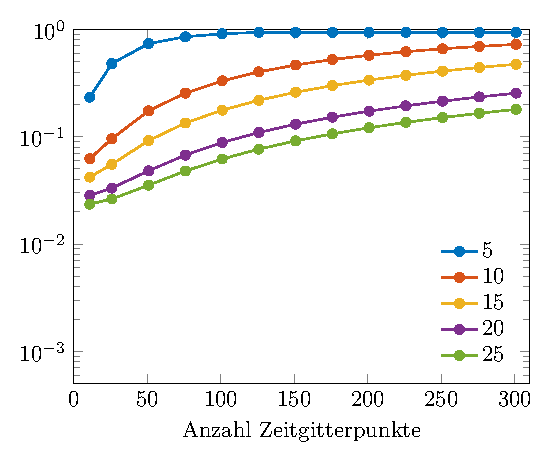
\includegraphics[width=1\textwidth]{figures/chapter4/infsup_homogen_ein_feld_a.pdf}
        \caption{Exakte inf-sup-Konstante $\beta_{\mathcal N}$.}
    \end{subfigure}
    ~
    \begin{subfigure}[b]{0.485\textwidth}
        \centering
        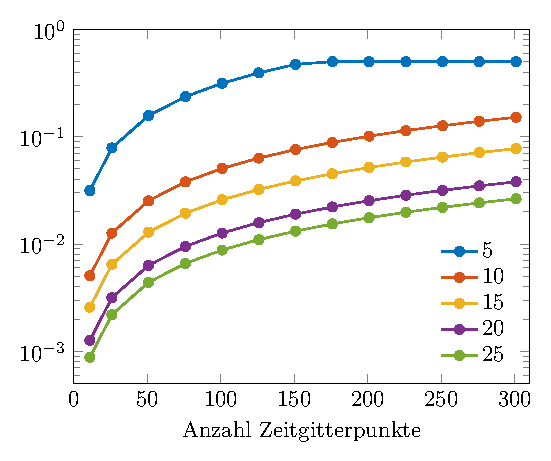
\includegraphics[width=1\textwidth]{figures/chapter4/infsup_homogen_ein_feld_b.pdf}
        \caption{Untere Schranke nach \cref{satz:untere_schranke_fuer_infsup_nach_andreev}.}
    \end{subfigure}
    \caption[Stabilität der Diskretisierung mit homogenen Randbedingungen, erstes Beispiel.]{%
        Zur Stabilität der Diskretisierung.
        Die Farben repräsentieren dabei die verschiedenen Werte für die Dimension $\mathcal J$ der räumlichen Diskretisierung $V_{\mathcal J}$.
        }
    \label{figure:infsup_homogen_ein_feld}
\end{figure}

\cref{figure:infsup_homogen_ein_feld} zeigt sowohl die exakt bestimmte diskrete inf-sup-Konstante $\beta_{\mathcal N}$ als auch die untere Schranke für verschiedene Werte von $\mathcal J$ und $\mathcal K$.
Zwar kann an dieser Stelle die Konstante $c_{0}$ aus \cref{satz:untere_schranke_fuer_infsup_nach_andreev} nicht näher bestimmt werden, aber es ist auf den ersten Blick ersichtlich, dass die Schranke das tatsächliche Verhalten der inf-sup-Konstante relativ gut widerspiegelt.
Ferner wird die CFL"=Bedingung bekräftigt, da für festes $\mathcal J$ und wachsende Anzahl $\mathcal K$ an Zeitgitterpunkten die inf"=sup"=Konstante sich dem Wert $1$ von unten annähert.

Das zweite, etwas komplexere Beispiel enthält nun einen zeitlichen Wechsel bei $T_{f} = 0.5$.
Der Differentialoperator $A(t) \colon V \to V'$ sei nun gegeben durch
\begin{equation}
    \begin{aligned}
        A(t)\eta =
        &- \Delta \eta + 3 \eta + \chi_{[0, 0.5)}(t) \left[ \sin(\pi \blank) - \sin(3 \pi \blank) \right] \eta
        \\&+ \chi_{[0.5, 1]}(t) \left[ \sin(2 \pi \blank ) + \sin(3 \pi \blank) \right] \eta.
    \end{aligned}
\end{equation}
Erneut ist mit $\mu = 3$ sichergestellt, dass die G\aa{}rding"=Ungleichung mit $\lambda = 0$ erfüllt wird.
\cref{figure:infsup_homogen_zwei_felder} zeigt die Ergebnisse für diese Modelldaten.
Auffallend ist, das die resultierenden Werte nahezu identisch sind mit denen des einfachen Beispiels, obwohl dies für die Modelldaten nur bedingt gilt.
Dies ist dadurch bedingt, dass in beiden Beispielen die Verschiebung $\mu$ so gewählt wurde, dass der Differentialoperator $A(t)$ elliptisch ist.

\begin{figure}[tb]
    \centering
    \centering
    \begin{subfigure}[b]{0.495\textwidth}
        \centering
        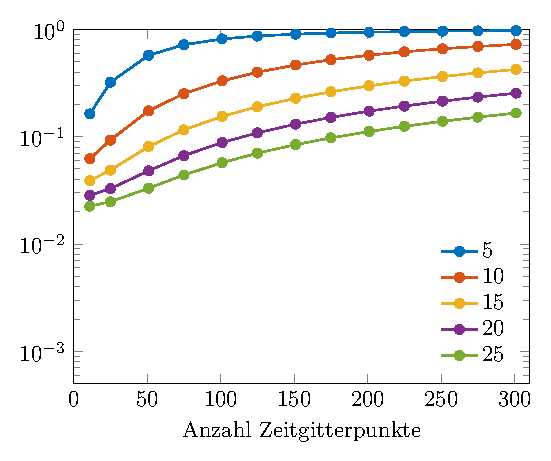
\includegraphics[width=1\textwidth]{figures/chapter4/infsup_homogen_zwei_felder_a.pdf}
        \caption{Exakte inf-sup-Konstante $\beta_{\mathcal N}$.}
    \end{subfigure}
    \begin{subfigure}[b]{0.495\textwidth}
        \centering
        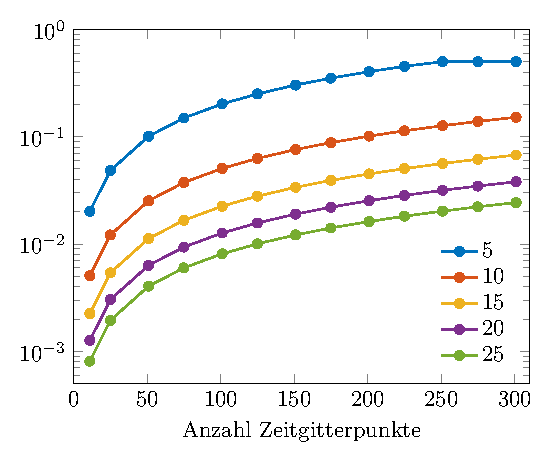
\includegraphics[width=1\textwidth]{figures/chapter4/infsup_homogen_zwei_felder_b.pdf}
        \caption{Untere Schranke nach \cref{satz:untere_schranke_fuer_infsup_nach_andreev}.}
    \end{subfigure}
    \caption[Stabilität der Diskretisierung mit homogenen Randbedingungen, zweites Beispiel.]{%
        Ergebnisse des zweiten Beispiels mit homogenen Randbedingungen.
        Erneut repräsentieren die Farben die verschiedenen Werte für $\mathcal J$.
        }
    \label{figure:infsup_homogen_zwei_felder}
\end{figure}

\paragraph{Periodische Randbedingungen.} % (fold)
\label{par:periodische_randbedingungen_}

Auch auf die periodischen Randbedingungen wollen an dieser Stelle kurz eingehen und das zweite Beispiel der homogenen Randbedingungen hier noch einmal betrachten.
Dabei übernehmen wir die dortigen Gegebenheiten und passen lediglich die verwendete Diskretisierung $V_{\mathcal J}$ an.
Diese wählen wir erneut in Form von Fourierfunktionen, diesmal als
\begin{equation}
    V_{\mathcal J} = \spn \Set{ v_{j} \given j = 1, \dots, \mathcal J}
\end{equation}
mit den Basisfunktionen
\begin{equation}
    v_{j} := \begin{cases}
        \cos(\pi (j - 1) \blank / L), & \text{falls } j \text{ ungerade},\\
        \sin(\pi j \blank / L), & \text{falls } j \text{ gerade}.
    \end{cases}
\end{equation}
Zwar können wir im Fall periodischer Randbedingungen mit den Aussagen in \cref{section:periodische_randbedingungen} nicht ohne Weiteres folgern, dass die G\aa{}rding-Ungleichung mit $\lambda = 0$ erfüllt wird, ... irgendwas?
Zwar können wir im periodischen Fall nicht ohne Weiteres die G\aa{}rding-Ungleichung mit $\lambda = 0$

\begin{figure}[tb]
    \centering
    \centering
    \begin{subfigure}[b]{0.495\textwidth}
        \centering
        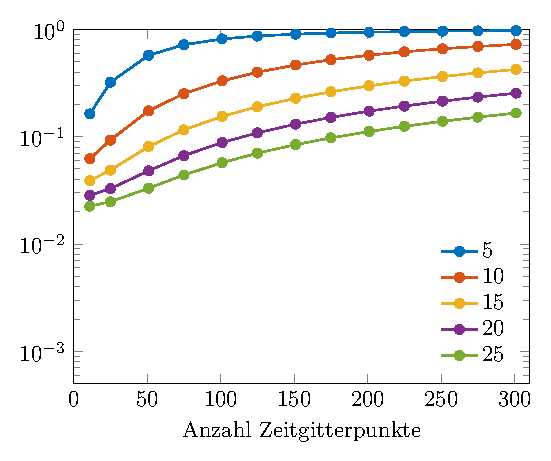
\includegraphics[width=1\textwidth]{figures/chapter4/infsup_homogen_zwei_felder_a.pdf}
        \caption{Exakte inf-sup-Konstante $\beta_{\mathcal N}$.}
    \end{subfigure}
    \begin{subfigure}[b]{0.495\textwidth}
        \centering
        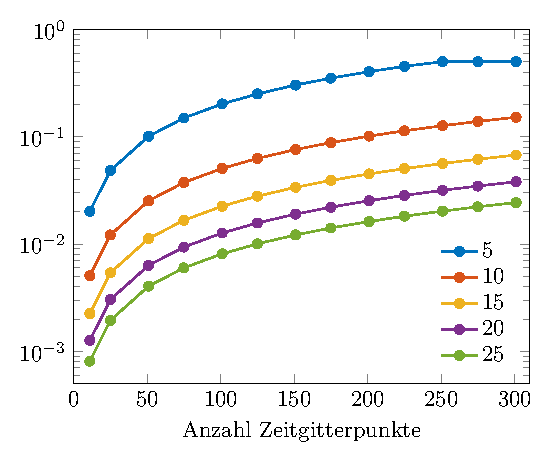
\includegraphics[width=1\textwidth]{figures/chapter4/infsup_homogen_zwei_felder_b.pdf}
        \caption{Untere Schranke nach \cref{satz:untere_schranke_fuer_infsup_nach_andreev}.}
    \end{subfigure}
    \caption[Stabilität der Diskretisierung mit homogenen Randbedingungen, zweites Beispiel.]{%
        Ergebnisse des zweiten Beispiels mit homogenen Randbedingungen.
        Erneut repräsentieren die Farben die verschiedenen Werte für $\mathcal J$.
        }
    \label{figure:infsup_periodisch_zwei_felder}
\end{figure}

% paragraph periodische_randbedingungen_ (end)

\end{document}
